% !TEX encoding = UTF-8 Unicode
\section{BLAS - Basic Linear Algebra Subprograms}
%%%%%%%%%%%%%%%%
	\begin{frame}{BLAS - Basic Linear Algebra Subprograms}{Levels}
		\begin{itemize}
			\item copy
			\item dot
			\item saxpy \\ \small $ z = \alpha x + y $ \normalsize
			\item gaxpy \\ \small $ z = Ax + y $ \normalsize
			\item matmul \\ \small  $ c = AB $ \normalsize
		\end{itemize}
		Level-1, Level-2, Level-3 $ \Rightarrow O(n), O(n^2), O(n^3)$
	\end{frame}
	\begin{frame}{Levels}
		\begin{enumerate}[a)]
			\item Level 1 BLAS vector-vector operations
			$y \leftarrow y + \alpha x$; dot products
			\begin{figure}
				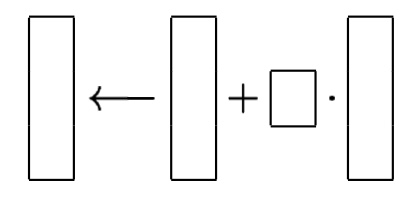
\includegraphics[height=1cm]{img/13/level1}
			\end{figure}
			\item Level 2 BLAS matrix-vector operations
			$y \leftarrow y + Ax$
			\begin{figure}
				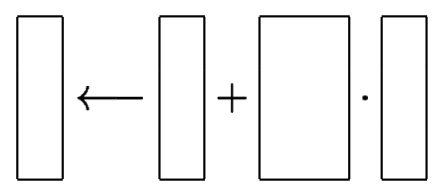
\includegraphics[height=1cm]{img/13/level2}
			\end{figure}
			\item Level 3 BLAS matrix-matrix operations
			$A \leftarrow A + B \cdot C$
			\begin{figure}
				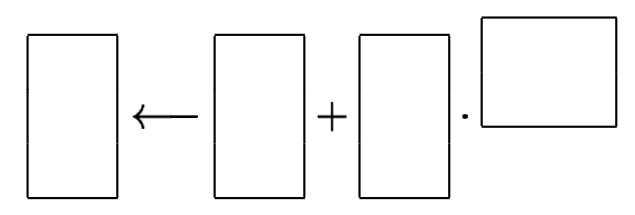
\includegraphics[height=1cm]{img/13/level3}
			\end{figure}
		\end{enumerate}
	\end{frame}
	\begin{frame}{Arithmetic/Memory references}
		Arithmetic is performed at the top of the memory hierarchy!!!
		\begin{figure}
			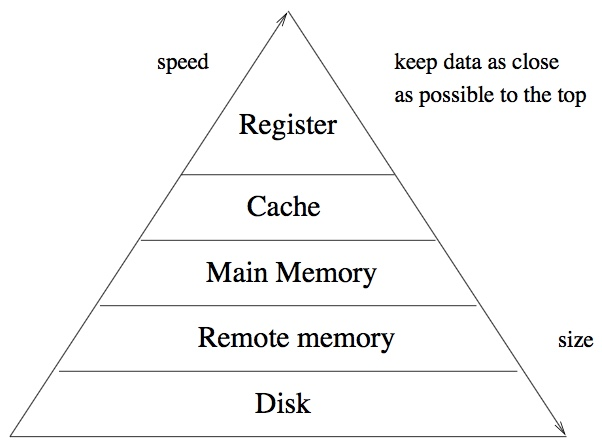
\includegraphics[height=5cm]{img/13/arithmeticmemref}
		\end{figure}
	\end{frame}
	\begin{frame}{Arithmetic/Memory references}
		\begin{tabular}{ | l | l | l | l | l |}
		\hline
		BLAS Level & 		& flops 	&memref 	& $\frac{flops}{mem ref}$ \\ \hline
		1 & $y \leftarrow y + \alpha x$ 	& $2n$ 	& $3n$ 	& $\frac{2}{3} $ \\ \hline
		2 & $y \leftarrow y + Ax$ 		& $2n^2$ 	& $n^2$ 	& 2 			\\ \hline
		3 & $C \leftarrow C + AB$ 	& $2n^3$ 	& $4n^2$ 	& $\frac{n}{2}$ 	\\ \hline
		\end{tabular} \\ 
		
		For level 1: 2 vector loads, 2 vector operations, 1 vector store\dots 
		
		Higher level: Increase of granularity $\Rightarrow$ lower synchronization cost
	\end{frame}
	\begin{frame}{BLAS character}
		\begin{itemize}
			\item \textit{clarity} - code $\rightarrow$ shorter, easier to read
			\item \textit{modularity} - programmers have larger building blocks
			\item \textit{performace} - manufacturers tuned machine-spec. BLAS
			\item \textit{program portability} - machine dependencies confined to the BLAS
		\end{itemize}
	\end{frame}
	\begin{frame}{BLAS naming conventions}
	\[
		\underbrace{1}_{} \underbrace{2}_{} \underbrace{3}_{} \underbrace{4}_{} \underbrace{5}_{} \underbrace{6}_{}
	\]
	1 $\rightarrow$ fortran data type of the matrix \\
	2, 3 $\rightarrow$ kind of the matrix involved \\
	4, 5, 6 $\rightarrow$ type of the operation
	\end{frame}
	